% !TeX spellcheck = en_US
%% 字体:方正静蕾简体
%%		 方正粗宋
\documentclass[a4paper,left=2.5cm,right=2.5cm,11pt]{article}

\usepackage[utf8]{inputenc}
\usepackage{fontspec}
\usepackage{cite}
\usepackage{xeCJK}
\usepackage{indentfirst}
\usepackage{titlesec}
\usepackage{longtable}
\usepackage{graphicx}
\usepackage{float}
\usepackage{rotating}
\usepackage{subfigure}
\usepackage{tabu}
\usepackage{amsmath}
\usepackage{setspace}
\usepackage{amsfonts}
\usepackage{appendix}
\usepackage{listings}
\usepackage{xcolor}
\usepackage{geometry}
\setcounter{secnumdepth}{4}
\usepackage{mhchem}
\usepackage{multirow}
\usepackage{extarrows}
\usepackage{hyperref}
\titleformat*{\section}{\LARGE}
\renewcommand\refname{参考文献}
\renewcommand{\abstractname}{\sihao \cjkfzcs 摘{  }要}
%\titleformat{\chapter}{\centering\bfseries\huge\wryh}{}{0.7em}{}{}
%\titleformat{\section}{\LARGE\bf}{\thesection}{1em}{}{}
\titleformat{\subsection}{\Large\bfseries}{\thesubsection}{1em}{}{}
\titleformat{\subsubsection}{\large\bfseries}{\thesubsubsection}{1em}{}{}
\renewcommand{\contentsname}{{\cjkfzcs \centerline{目{  } 录}}}
\setCJKfamilyfont{cjkhwxk}{STXingkai}
\setCJKfamilyfont{cjkfzcs}{STSongti-SC-Regular}
% \setCJKfamilyfont{cjkhwxk}{华文行楷}
% \setCJKfamilyfont{cjkfzcs}{方正粗宋简体}
\newcommand*{\cjkfzcs}{\CJKfamily{cjkfzcs}}
\newcommand*{\cjkhwxk}{\CJKfamily{cjkhwxk}}
\newfontfamily\wryh{Microsoft YaHei}
\newfontfamily\hwzs{STZhongsong}
\newfontfamily\hwst{STSong}
\newfontfamily\hwfs{STFangsong}
\newfontfamily\jljt{MicrosoftYaHei}
\newfontfamily\hwxk{STXingkai}
% \newfontfamily\hwzs{华文中宋}
% \newfontfamily\hwst{华文宋体}
% \newfontfamily\hwfs{华文仿宋}
% \newfontfamily\jljt{方正静蕾简体}
% \newfontfamily\hwxk{华文行楷}
\newcommand{\verylarge}{\fontsize{60pt}{\baselineskip}\selectfont}  
\newcommand{\chuhao}{\fontsize{44.9pt}{\baselineskip}\selectfont}  
\newcommand{\xiaochu}{\fontsize{38.5pt}{\baselineskip}\selectfont}  
\newcommand{\yihao}{\fontsize{27.8pt}{\baselineskip}\selectfont}  
\newcommand{\xiaoyi}{\fontsize{25.7pt}{\baselineskip}\selectfont}  
\newcommand{\erhao}{\fontsize{23.5pt}{\baselineskip}\selectfont}  
\newcommand{\xiaoerhao}{\fontsize{19.3pt}{\baselineskip}\selectfont} 
\newcommand{\sihao}{\fontsize{14pt}{\baselineskip}\selectfont}      % 字号设置  
\newcommand{\xiaosihao}{\fontsize{12pt}{\baselineskip}\selectfont}  % 字号设置  
\newcommand{\wuhao}{\fontsize{10.5pt}{\baselineskip}\selectfont}    % 字号设置  
\newcommand{\xiaowuhao}{\fontsize{9pt}{\baselineskip}\selectfont}   % 字号设置  
\newcommand{\liuhao}{\fontsize{7.875pt}{\baselineskip}\selectfont}  % 字号设置  
\newcommand{\qihao}{\fontsize{5.25pt}{\baselineskip}\selectfont}    % 字号设置 

\usepackage{diagbox}
\usepackage{multirow}
\boldmath
\XeTeXlinebreaklocale "zh"
\XeTeXlinebreakskip = 0pt plus 1pt minus 0.1pt
\definecolor{cred}{rgb}{0.8,0.8,0.8}
\definecolor{cgreen}{rgb}{0,0.3,0}
\definecolor{cpurple}{rgb}{0.5,0,0.35}
\definecolor{cdocblue}{rgb}{0,0,0.3}
\definecolor{cdark}{rgb}{0.95,1.0,1.0}
\lstset{
	language=[x86masm]Assembler,
	numbers=left,
	numberstyle=\tiny\color{black},
	showspaces=false,
	showstringspaces=false,
	basicstyle=\scriptsize,
	keywordstyle=\color{purple},
	commentstyle=\itshape\color{cgreen},
	stringstyle=\color{blue},
	frame=lines,
	% escapeinside=``,
	extendedchars=true, 
	xleftmargin=1em,
	xrightmargin=1em, 
	backgroundcolor=\color{cred},
	aboveskip=1em,
	breaklines=true,
	tabsize=4
} 

\newfontfamily{\consolas}{Consolas}
\newfontfamily{\monaco}{Monaco}
\setmonofont[Mapping={}]{Consolas}	%英文引号之类的正常显示,相当于设置英文字体
\setsansfont{Consolas} %设置英文字体 Monaco, Consolas,  Fantasque Sans Mono
\setmainfont{Times New Roman}

\setCJKmainfont{华文中宋}


\newcommand{\fic}[1]{\begin{figure}[H]
		\center
		\includegraphics[width=0.8\textwidth]{#1}
	\end{figure}}
	
\newcommand{\sizedfic}[2]{\begin{figure}[H]
		\center
		\includegraphics[width=#1\textwidth]{#2}
	\end{figure}}

\newcommand{\codefile}[1]{\lstinputlisting{#1}}

% 改变段间隔
\setlength{\parskip}{0.2em}
\linespread{1.1}

\usepackage{lastpage}
\usepackage{fancyhdr}
\pagestyle{fancy}
\lhead{\space \qquad \space}
\chead{第三次学习报告 \qquad}
\rhead{\qquad\thepage/\pageref{LastPage}}
\begin{document}

\tableofcontents

\clearpage

\section{中断和异常处理}
\subsection{异常和异常处理}
处理器为了实现处理异常和中断,使用了一个数据结构,也就是中断描述符表,用于存放中断描述符。同时处理器为每个异常和中断条件都赋予了一个向量,用于作为中断描述符表的索引号。\par
	中断可以从硬件和软件产生。外部中断通过INTR和NMI接收。NMI接收的中断是不可屏蔽中断,其向量号为2。INTR接收的外部中断可屏蔽,通过设置EFLAGS中的IF位为0来屏蔽这些中断。这里的IF标志可以通过STI和CLI来设置或清零。只有当程序的CPL(程序特权级)小于IOPL(I/O特权级字段)时,才可执行这两条指令。还有几种情况可以影响IF标志,比如PUSHF指令、IRET指令等。当通过中断门处理一个中断时,IF会被自动清零。\par
	软件中断主要借助INT指令,在指令操作数中提供中断向量号。向量号0到255都可以作为INT指令的中断号,比如指令INT 0x80可以执行系统中断。EFLAGS中的IF标志无法屏蔽软件中断。\par

\subsection{IDT和IDT描述符}
中断描述符表类似于全局描述符表,用于存放门描述符。处理器使用IDTR寄存器定位IDT表的位置,IDTR有48位,高32位是IDT表的基地址,而低16位为IDT的长度值。使用LIDT指令可以将内存中的基地址和限长值加载到IDTR寄存器中,不过该指令只能由CPL为0的代码执行。\par
	IDT存放的门描述符有三类,为中断门描述符、陷阱门描述符和任务门描述符,它们都是8字节的。中断门描述符和陷阱门描述符中存放了段选择符和偏移值,用于对段的寻址,从而将程序执行权转移到代码段中异常或中断的处理过程中。而任务门描述符中含有段选择符,不过没有偏移值,因为在门中的偏移值没有意义。\par

\subsection{异常与中断处理}
	发生异常或中断时,处理器使用异常或中断的向量作为IDT表的索引,从而得到相应的门描述符。门描述符中的段选择符指向GDT或IDT中的段描述符,而段描述符给出相应代码段的段基址。门描述符中的偏移值作为段基址的偏移,从而指向执行异常或中断处理过程的代码段。我觉得下面这张图描述得很形象。\par
	\begin{figure}[H]
		\center
		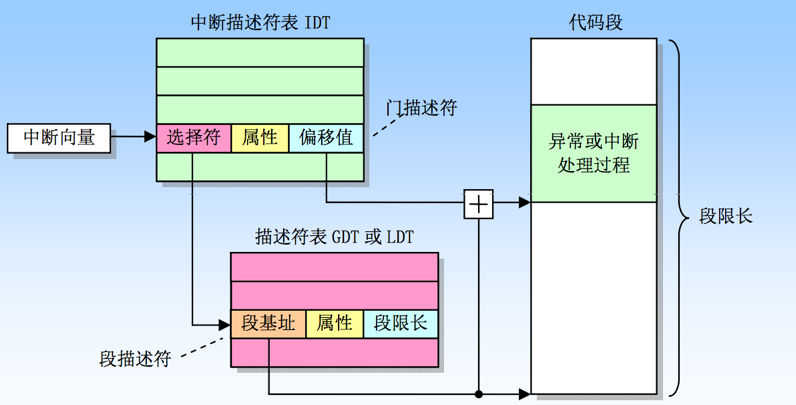
\includegraphics[width=0.53\textwidth]{1.png}
	\end{figure}
	
	异常或中断处理分为两种情况。一种是在高特权级下执行,一种是在同一特权级下执行。\par
		处理过程在高特权级上执行时,将会发生堆栈切换操作。此时处理器首先获得新栈的段选择符SS和栈指针ESP,这里的段选择符和栈指针由当前任务的TSS段提供。然后把原栈选择符和栈指针压入新栈。随后将EFLAGS、CS和EIP当前值压入新栈。如果异常会产生一个错误号,该错误号也将被压入新栈。如下图所示。\par
	\begin{figure}[H]
		\center
		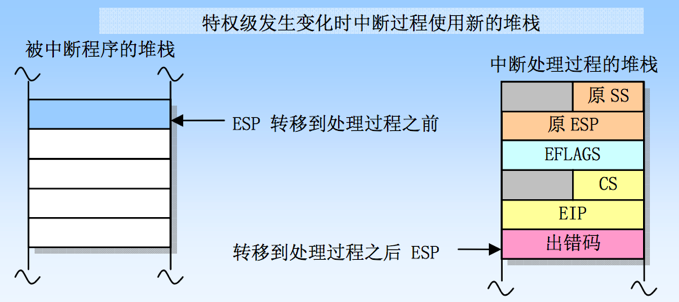
\includegraphics[width=0.6\textwidth]{2.png}
	\end{figure}
	
	处理过程在同一特权级上执行时,过程相对简单。处理器将EFLAGS、CS和EIP当前值压入堆栈。如果异常会产生一个错误号,该错误号也会被压入堆栈。这个过程如下图所示。\par
	\begin{figure}[H]
		\center
		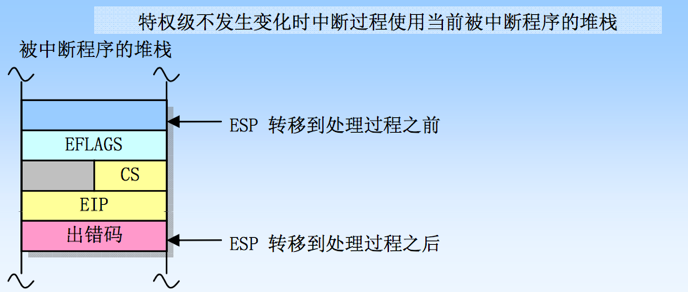
\includegraphics[width=0.6\textwidth]{3.png}
	\end{figure}
	
	中断处理过程结束时,程序使用IRET指令从中断处理过程中返回。此时处理器会从堆栈中弹出代码段的选择符CS和指令指针EIP。同时IRET会把保存的寄存器内容恢复到EFLAGS中。在特权级保护机制下,只有当CPL为0时,IOPL字段才会被恢复。只有CPL小等于IOPL时,IF标志才会被改变。如果中断处理过程中发生了堆栈切换,那么IRET指令会切换回原来的堆栈。\par
		需要注意的是,通过中断门访问异常或中断处理过程时,处理器会清零IF标志,随后再使用IRET指令恢复IF标志。而通过陷阱门访问处理过程则不会影响IF标志。\par

\subsection{错误码}
	错误码类似于段选择符,用于寻址段。不过这里的段是与特定的异常条件有关的。段错误码的格式如下所示。\par
	\begin{figure}[H]
		\center
		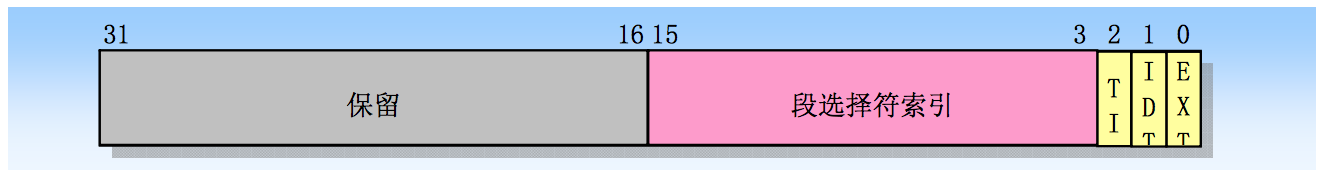
\includegraphics[width=0.5\textwidth]{4.png}
	\end{figure}
	
	图中的低三位为TI、IDT和EXT。EXT为0时,表示执行程序以外的事件造成了异常。IDT为0时,错误码的索引指向GDT或LDT的段描述符;当IDT为1时,错误码的索引指向IDT的一个门描述符。只有当TI为0时TI标志才有用。因为TI标志用于选择GDT表和LDT表。当TI为1时,错误码的索引部分指向LDT的段描述符;当TI为0时,错误码的索引部分指向GDT表中的描述符。\par
	错误码有一个特例,也就是页故障异常的错误码。页故障错误码中没有段选择符索引,只有最低3位比特位有效,分别为P、W/R和U/S。P=0时,表示也不存在;P为1时,表示违反页级保护权限。W/R=0时,表示读操作引起了异常;W/R=1时,表示异常由写操作引起。U/S=0时,表示异常发生时CPU正在执行超级用户代码;U/S=1时,表示异常发生时CPU正在执行一般用户代码。在第一次学习报告有提到过,CR2控制寄存器中存放着引起页面故障异常的线性地址。\par

\section{任务管理}
\subsection{用于任务管理的数据结构}
	为了进行任务管理,处理器定义了一些寄存器和数据结构,分别为任务状态段TSS、TSS描述符、任务寄存器TR和任务门描述符。\par
	用于恢复一个任务执行的处理器状态信息被保存在TSS中。TSS分为两类字段,一个是动态字段,还有一个是静态字段。当任务切换而被挂起时,处理器会更新动态字段的内容。而静态字段通常不会改变,它的字段内容在任务被创建时设置。\par
	TSS由任务状态段描述符来寻址和定义,以下是TSS段描述符的格式。
	\fic{5.png}
	
	描述符中的TYPE字段中的B标志用于表示任务是否处于忙状态。B=1时,表示任务正忙;B=0时,表示任务处于非活动状态。描述符中的G标志是颗粒度,当G=0时,TSS段的长度必须大等于104字节。描述符中的DPL标志用于特权级保护机制中。当发生任务切换时,访问TSS的程序的CPL必须小等于TSS中的DPL。描述符中的段基址就是任务状态段的基址。\par
	任务寄存器存放着段选择符和当前TSS段描述符。LTR指令可以在系统初始化阶段给TR寄存器加载初值,之后TR的内容会在任务切换时自动地被改变。\par
	除了使用段选择符直接访问GDT中的TSS描述符,还可以通过任务门描述符间接地访问TSS描述符,因为任务门描述符含有TSS选择符字段。任务门描述符中的DPL用于支持特权级保护机制。当程序通过任务门描述符调用程序时,程序的CPL以及指向任务门描述符的门选择符的RPL都必须小等于任务门描述符中的DPL。\par
	下图描述了调用任务的两种方式,一种是通过任务门描述符访问,一种是通过TSS段描述符访问。从图中可以看出,任务门描述符可以存放在GDT、LDT或IDT表中,程序通过任务门描述符间接访问到TSS描述符。
	\fic{6.png}
\subsection{任务切换}
	处理器可以通过4种方式进行任务切换操作,分别是:1.对TSS描述符执行JMP或CALL指令。2.对任务门描述符执行JMP或CALL指令。3.通过中断或异常向量指向任务门描述符。4.执行IRET指令。\par
	以下是进行任务切换的过程:
	\begin{itemize}
		\item 首先获得新任务的TSS段选择符。段选择符的获取有三种途径:1.从JMP或CALL指令操作数中获取。2.中断向量索引到IDT表中的任务门描述符,获取其中的TSS选择符。3.执行IRET指令时,从当前TSS的前一任务链接字段中获取。\par
		这里说一下前一任务链接字段,它需要和EFLAGS中的NT标志配合使用。NT标志为1时,表明当前任务嵌套在另一个任务中执行,并且当前任务的TSS段的前一任务链接字段中存放着高一层任务的TSS选择符。
		\item 经过特权级保护机制的检查。使用JMP或CALL调用程序时,当前任务的CPL和新任务的TSS段选择符的RPL必须小等于新任务TSS段描述符的DPL。发生中断、异常或使用IRET指令时,则无视特权级保护机制。
		\item 对B标志和NT标志的设置。如果使用JMP进行任务切换,则将B标志清零。如果使用IRET指令进行任务切换,则将B标志和NT标志清零。
		\item 将当前任务状态保存到当前任务的TSS中,包括所有通用寄存器的值,段寄存器中的段选择符,标志寄存器EFLAGS以及指令指针EIP。
		\item 加载新的TSS段描述符。如果任务切换由CALL、JMP、异常或者中断产生,则对新TSS段描述符中的B标志置1。
		\item 将新TSS的段选择符和描述符加载到任务寄存器中。同时设置CR0寄存器的任务已切换标志TS为1。
		\item 将新TSS状态加载进处理器,包括所有通用寄存器、段选择符、标志寄存器EFLAGS、LDTR寄存器、CR3寄存器以及EIP。如果任务切换由CALL、JMP、异常或者中断产生,则将EFLAGS中的NT位置一。
		\item 开始执行新任务。
	\end{itemize}
\subsection{任务地址空间}
	任务的地址空间由任务能够访问的段构成,这些段有代码段、数据段、堆栈段、TSS中引用的系统段以及任务代码能够访问的任何其他段。\par
	在任务之间共享数据有以下三个途径:
	\begin{itemize}
		\item 通过GDT共享数据。这个方法是很明显而且简单的。不同的段可以映射到相同的物理地址空间中,而每个段又有对应的段描述符。这些段描述符存放在GDT表中。于是任务通过GDT共享相同的物理地址空间。这种方法的缺点是所有任务都可以共享这些段中的代码和数据。
		\item 让任务共享相同的LDT。让一些特定的任务的TSS中LDT字段指向同一个LDT,从而访问到相同的物理地址空间。
		\item 让不同LDT中的某些段描述符映射到相同的物理地址。这样的段描述符通常被称为别名段。
	\end{itemize}
\section{编写保护模式}
\subsection{从实模式跳转到保护模式}
	首先定义段描述符的数据结构。根据X86下的段描述符通用格式可知,段描述符都是64位的,也就是8字节。
	\begin{lstlisting}
		%macro  Descriptor  3
		        dw  %2 & 0FFFFh ; dw = define word 段限长1
		        dw  %1 & 0FFFFh ; 段基址1
		        db  (%1 >> 16) & 0FFh ; db = define byte 段基址2
		        dw  ((%2 >> 8) & 0F00h) | (%3 & 0F0FFh) ; 属性1+段限长2+属性2 
		        db  (%1 >> 24) & 0FFh ; 段基址3
		%endmacro
	\end{lstlisting}
	
	定义这个数据结构的时候,使用了多行宏。多行宏的格式如下:
	\begin{lstlisting}
		%macro prologue 1 ; 这里的数字1定义了可以接收的参数个数
			push	ebp
			mov		ebp,esp
			sub     esp,%1 ; 用于引用宏调用中的第一个参数
		%endmacro
	\end{lstlisting}
	
	现在回过头来看描述符的格式,之所以将它定义为这样的格式,是为了遵照X86中的段描述符通用格式,见下图。
	\sizedfic{0.8}{7.png}
	
	接着我们需要写gdt的段。这个段定义GDT描述符表。正如上一份学习报告所写的,GDT描述符表是一个存放段描述符的数组。
	\begin{lstlisting}
		[SECTION .gdt]
		
		; GDT描述符表
		; 描述符第一个参数是段基址
		LABEL_GDT:          Descriptor  0,      0,                  0
		; 由于32位代码段的段基址在此无法确定,所以先设为0,之后再初始化
		LABEL_DESC_CODE32:  Descriptor  0,      SegCode32Len - 1,   DA_C + DA_32
		; 这个段描述符指向的是显存
		LABEL_DESC_VIDEO:   Descriptor  0B8000h,0ffffh,             DA_DRW
		
		; GDT表的长度,nasm中$代表当前行相对于段基址的偏移地址
		GdtLen  equ $ - LABEL_GDT 
		
		; GdtPtr的前2两个字节为GDT表的边界,后4个字节是GDT表的基地址
		GdtPtr  dw  GdtLen - 1
		        dd  0 ; define double-word
		
		; 以下是两个段选择符,用于索引GDT表中的段描述符
		SelectorCode32  equ LABEL_DESC_CODE32 - LABEL_GDT
		SelectorVideo   equ LABEL_DESC_VIDEO - LABEL_GDT
	\end{lstlisting}
	
	接下来我们要编写[SECTION .s16]的代码段,这是个16位代码段。我使用这个代码段跳转进入保护模式。\par
	在给出代码之前,我想说一下为什么需要定义一个16位的代码段。首先要知道,在16位代码段中,跳转目标的偏移用16位表示。其次还要认识到,CPU还处在实模式下。在实模式下,CPU总是进行16位的跳转,也就是当他在解析跳转目标的时候,总是读取内存中的16位的值作为跳转目标。为此,汇编器要配合CPU,产生这种用16位表示偏移量的代码。\par
	下面就是我要写的16位代码段。
	\begin{lstlisting}
		[SECTION .s16]
		[BITS 16] ; 告诉编译器这个段需要按照16位进行编译
		LABEL_BEGIN:
			; cs存放着cpu执行的代码段的基地址
			; 初始化寄存器中的值
		    mov ax,cs
		    mov ds,ax
		    mov es,ax
		    mov ss,ax
		    mov sp,0100h
			
			; 初始化LABEL_DESC_CODE32描述符
		    xor eax,eax ; 将eax中的值清零
		    mov ax,cs
			; 下面两句相当于cs*16+偏移地址
		    shl eax,4
		    add eax,LABEL_SEG_CODE32
			; 这样eax里就存放着32位代码段的物理地址
			; 接下来4条语句分别初始化了32位代码段描述符的基地址1、基地址2和基地址3
			; 要注意段描述符是8字节,这样会比较好理解代码
		    mov word [LABEL_DESC_CODE32 + 2], ax
		    shr eax,16
		    mov byte [LABEL_DESC_CODE32 + 4], al
		    mov byte [LABEL_DESC_CODE32 + 7], ah
			
			; 为加载GDTR作准备
		    xor eax,eax  ; 将eax中的值清零
		    mov ax,ds
			; 下面两句得到了GDT表在代码段中的物理地址
		    shl eax,4
		    add eax,LABEL_GDT
			; 初始化指向GDT表的指针,修改GdtPtr中的GDT基地址
		    mov dword [GdtPtr + 2], eax
			
			; 关闭中断
		    cli
			
			; 加载GdtPtr到寄存器gdtr
		    lgdt [GdtPtr]
			
			; 打开地址线A20
		    in  al,92h
		    or  al,00000010b
		    out 92h,al
			
			; 准备切换到保护模式
			; 将cr0的第0位设为1。cr0的第0位是PE位,PE=1时,CPU运行于保护模式。
		    mov eax,cr0
		    or  eax,1
		    mov cr0,eax
			
			; 真正进入到保护模式
		    jmp dword SelectorCode32:0
	\end{lstlisting}
	
	上述代码的注释虽然已经描述得很详细,但我觉得还是有必要完整得叙述一遍从实模式切换到保护模式的过程。
	\begin{itemize}
		\item 首先初始化一些起码的系统数据结构,比如GDT表和一个代码段。
		\item 禁止中断,这是为了确保在模式切换操作期间不产生异常和中断。
		\item 执行LGDT指令把GDT表的基地址加载进入GDTR寄存器。
		\item 将控制寄存器CR0中的PE标志置一。
		\item 进入保护模式。
	\end{itemize}
	
	接下来编写32位代码段。类似于16位代码段,在32位代码段中,跳转目标的偏移用32位表示。\par
	\begin{lstlisting}
		[SECTION .s32]
		[BITS 32] ; 告诉编译器这个段需要按照32位进行编译

		LABEL_SEG_CODE32:
		    mov ax, SelectorVideo
			; gs是80386起增加的辅助段寄存器
			; gs目前存放了LABEL_DESC_VIDEO段描述符对应的段选择符
		    mov gs, ax
		    mov edi, (S0 * l1 + 79) * 2
		    mov ah, 0Ch
		    mov al, 'P'
			; 逻辑地址gs:edi,经过段机制后转化为线性地址,为LABEL_DESC_VIDEO偏移edi位
			; 将ax的值写入显存中偏移edi的位置
		    mov [gs:edi], ax
		    jmp $

		SegCode32Len equ $ - LABEL_SEG_CODE32
	\end{lstlisting}
	
	虽然上一次学习报告已经提到过段机制,但是因为比较简略,所以在此我附上一张段式寻址方式的图加以说明。
	\fic{8.png}

\subsection{从保护模式跳转到实模式}
	如果想要切换回实地址模式,需要按照下面的步骤:
	\begin{itemize}
		\item 首先禁止中断。
		\item 把程序的控制转移到长度为64KB的可读段中。这步操作使用实模式要求的段长度加载CS寄存器。
		\item 使用一个特殊定义的选择符来加载SS、DS、ES、FS和GS段寄存器,这个选择符指向的段描述符段限长为64KB,颗粒度为字节,向上扩展,可写,且存在于内存中。
		\item 清除CR0中的PE标志。
		\item 执行一个远跳转指令跳转到实模式程序中。
		\item 加载实地址模式代码会使用的SS、DS、ES、FS和GS寄存器。
	\end{itemize}
	
	相应的代码如下,需要注意的是,跳转回实模式的代码需要在16位代码段中完成。
	\begin{lstlisting}
		LABEL_GDT: Descriptor 0,0,0
		LABEL_DESC_NORMAL: Descriptor 0,0ffffh,DA_DRW
		
		SelectorNormal equ LABEL_DESC_NORMAL-LABEL_GDT
		
		[SECTION .s16code]
		[BITS 16]
		LABEL_SEG_CODE16:
			cli
			; 使用一个特殊定义的选择符来加载SS、DS、ES、FS和GS段寄存器
			mov ax,SelectorNormal
			mov ds,ax
			mov es,ax
			mov fs,ax
			mov gs,ax
			mov ss,ax
			
			mov eax,cr0
			and al,11111110b
			mov cr0,eax
		
			mov ax,cs
			mov es,ax
			mov ds,ax
			mov ss,ax
			
			; 这里的SPValueInRealMode是在16位代码段初始化时赋值的
			mov sp,[SPValueInRealMode]
			
			in al,92h
			and al,11111101b
			out 92h,al
			
			sti
		Code16Len equ $-LABEL_SEG_CODE16
	\end{lstlisting}

\subsection{完整的例子}
	我阅读了一个完整的例子,自己能理解它的意思,也把自己所理解的注释写在代码中了。看完这个例子,我有自信自己可以写出引导区代码是如何让操作系统从保护模式跳转到实模式,以及让操作系统从实模式跳转回保护模式。\par
	在看代码之前,我觉得有必要先了解一些X86中的段寄存器
	\begin{itemize}
		\item x86的段寄存器有CS寄存器、DS寄存器、SS寄存器、ES寄存器、FS以及GS寄存器。CS寄存器存放着程序代码段的基地址。DS寄存器存放着程序数据段的基地址。SS寄存器堆栈段的基地址。ES、FS和GS寄存器是扩展寄存器,用于内存寻址,常与变址寄存器配合使用。
		\item x86的指针寄存器有IP寄存器、SP寄存器和BP寄存器。IP寄存器常与CS配合,用于寻址下一条要执行的指令。SP寄存器常与SS配合,用于寻址堆栈中的数据。BP寄存器是一个扩展寄存器。
		\item x86的通用寄存器有AX寄存器、BX寄存器、CX寄存器和DX寄存器。AX寄存器用于输入输出以及大部分的算术运算。BX寄存器是主要的基址寄存器,用于和变址寄存器配合。CX寄存器是计数寄存器。DX寄存器是数据寄存器。
		\item x86的变址寄存器有SI寄存器和DI寄存器。SI寄存器是源变址寄存器,DI是目的变址寄存器。
	\end{itemize}
	
	为了更好的理解代码,我还去了解了EFLAGS标志寄存器中的各个标志位。
	\begin{itemize}
		\item 进位标志CF。这个标志用于反映运算是否产生进位或借位。
		\item 奇偶标志PF。用于反映运算结果中1的个数的奇偶性。
		\item 辅助进位标志AF。在字操作时,发生低字节向高字节进位或借位时,AF=1。在字节操作时,发生低4位向高4位进位或借位时,AF=1。
		\item 零标志ZF。用于反映运算结果是否为0。
		\item 符号标志SF。用于反映运算结果的符号位。
		\item 溢出标志OF。用于反映有符号数加减所得结果是否溢出。
		\item 追踪标志TF。TF=1时,CPU进入单步执行方式。
		\item 中断允许标志IF。用于决定CPU是否响应CPU外部的可屏蔽中断发出的中断请求。
		\item 方向标志DF。用于决定在串操作指令执行时有关指针寄存器发生调整的方向。
		\item IOPL标志位,也就是I/O特权级字段。
		\item 嵌套任务标志NT,这在之前有提到过。
		\item 重启动标志RF,用于控制是否接收调试故障。
		\item 虚拟8086方式标志VM。VM=1时,表示处理机处于虚拟的8086方式下的工作状态。
	\end{itemize}
	
	下图是标志寄存器EFLAGS。
	\fic{9.png}
	
	下面就是我所读的代码。我在linux上调试了这段代码,不过由于是在另外一台电脑上,所以就不附上调试过程了。
	\codefile{pmtest2.asm}
	
\end{document}
